% \addcontentsline{toc}{chapter}{Problem Implementation}
\chapter{Problem Implementation}
\oddsidemargin = -30pt

\section{Grammar}

\noindent For a better understanding, further is represented the grammar for this specific language according to a very simple and textual program. Through it, was shown in detail each feature of grammar.
The DSL design includes several stages. First of all, definition of the programming
language grammar  
G = (VN,VT, P, S ):

VN – is a finite set of non-terminal symbol;

VT - is a finite set of terminal symbols.

P – is a finite set of production of rules;

S - is the start symbol;\\

$VN = {<program>, <var>, <knot>, <ID>, <content>, <text>, <goto>, <print>,$
$<img>, <choice>, <var_op>, <expr>, <int>, <str>, <value>, <var_name>, $
$<knot_name>, <img_name>, <option_text>, <EQ>, <LPAREN>, <RPAREN>, <LCURLY>, $
$<RCURLY>, <GH>, <EXLAM>, <IMG_NAME>, <INT>, <ID>, <WS>, <EOF>} $

$VT = {'EOF', '(', ')', '*', '=', '<', '>', '[', ']', '{', '}', '!', '+', '-', '/', '(', ')(', ')', '<', '>', '=', '[', ']', '!', a'{', '}', ',', $
$'.png', '.jpg', ‘0’..’9’, ‘a..z’, ‘A’..’Z’}$

\noindent In Table 1 are meta-notations used for specifying the grammar. 
\begin{table}[h]
    \centering
    %\caption{Meta notation} C-c
    \begin{tabular}{|c|c|}
        \hline
        Notation (symbol) & Meaning\\
        \cline{1-2}
        $<foo>$ & means foo is a nonterminal\\
        \hline
        foo & foo in bold means foo is a terminal\\
        \hline
        x* & zero or more occurrences of x\\
        \hline
        $|$ & separates alternatives\\
        \hline
        → & derives\\
        \hline
        // & comment section\\
        \hline
    \end{tabular}
    \label{tbl:epochs}
\end{table} \\
\begin{verbatim}
        grammar Expr;
        
        <program>: (<var>)* <knot>+ EOF;
        
        <knot> : <ID> '{' <content>* '}'; 
        <var>: <var_name> '=' <value>;
        <value>: <int>|<str>;
        <int>:<INT>;
        <str>:'"'(<ID>|<INT>)*'"';
        
        
        <content>: <text>
            | <goto>
            | <print>
            | <npc>
            | <choice>
            | <var_op>
            | <if>
            ;
        
        <var_op> : '[' <var_name> '=' <expr> ']';
        <if> : '(' '(' '?' <logic_expr> <goto> ')'')';
        
        <logic_expr>: <logic_expr> ('&''&'|'|''|') <logic_expr>
                   | '(' <logic_expr> ')'
                   | <bool_expr>
                    ;
        <bool_expr>: <bool_expr> ('>'|'<'|'!''='|'=''='|'>''='|'<''=') <bool_expr>
                   | <expr>
                   ;
        
        <expr>:   <expr> ('*'|'/') <expr>
            |   <expr> ('+'|'-') <expr>
            |   <int>
            |   '(' <expr> ')'
            |   <str>
            | <var_name>
            ;
        
        <goto> : '(' <knot_name> ')' ;
        <print> : '(''(' <var_name> ')'')';
        <npc>: '(''!' (<text>)+ ')';
        <choice>: '(' '(' <pair*>  ')'')';
        <pair>:'!'(<text>)+ <goto>;
        <knot_name>: <ID>;
        <var_name>:<ID>|<INT>;
        <text>: <ID>|<INT>;
        
        <EQ> : '=' ;
        <LPAREN> : '('; 
        <RPAREN> : ')' ;
        <LCURLY> : '{' ;
        <RCURLY> : '}' ;
        <GH>:'"';
        <EXLAM>: '!';
        <L>: '[';
        <R>: ']';
        <MULT>: '*';
        <DIVIDE>: '/';
        <SUB>: '-';
        <ADD>: '+';
        
        INT : [0-9]+ ;
        ID: [a-zA-Z_0-9?.\\,;%<>!]+; 
        WS: [ \t\n\r\f]+ -> skip ;
\end{verbatim}


\section{Semantic and lexicon}
\noindent The grammar provided is a context-free grammar (CFG) that defines the syntax rules for an interactive story telling program. Here are the descriptions of the semantic and lexicon of the grammar:\\
Semantic:
\begin{itemize}
        \item $<program>$ is the starting point of the program, which consists of a series of $<var>$ declarations followed by one or more $<knot>$ definitions.
        \item $<knot>$ defines a scene or a chapter in the story, identified by an $<ID>$ (identifier) followed by a block of $<content>$ that can be a sequence of text, choices, images, variables, and go-to statements.
        \item $<var>$ declares a variable with a $<var_name>$ identifier and assigns a $<value>$ to it, where a value can be either an integer or a string.
        \item $<var_op>$ is an expression that can update the value of a variable by performing basic arithmetic operations on it.
        \item $<expr>$ is an arithmetic expression that can include integers, strings, and variables. \\
\end{itemize}
Lexicon:
\begin{itemize}
        \item $<INT>$ is a regular expression that represents any positive integer number.
        \item $<ID>$ is a regular expression that represents an identifier or a name, starting with an alphabetical character or an underscore and followed by alphanumeric characters or underscores.
        \item $<IMG_NAME>$ is a regular expression that represents the name of an image file in the PNG or JPG format.
        \item $<WS>$ is a regular expression that matches any whitespace character and is ignored by the parser.
        \item $<EQ>, <LPAREN>, <RPAREN>, <LCURLY>, <RCURLY>, <GH>, and <EXLAM>$ are tokens that represent the symbols "=","(",")","{","}","""","!" respectively, used to separate and define the syntax rules of the grammar.
\end{itemize}

\section{Syntax Analysis}
Writing syntax analysis for an interactive storytelling language involves creating a grammar that defines the language's syntax and using it to parse input text to ensure it conforms to the grammar rules. We started by defining the language’s grammar, then we generated the parser, using ANTLR, that was able to read and interpret the input text according to the grammar rules. Afterwards the parser has successfully recognized a valid input, it needs to perform semantic actions based on the syntax to actually execute the code. This involves interpreting the input and manipulating variables, objects, or other data structures as necessary. For our interactive storytelling language, these semantic actions were changing the storyline based on user choices or triggering events based on certain input. Therefore, we had only to handle the errors, test and refine the grammar and parser as needed to improve accuracy of performance.

Creating syntax analysis for our interactive storytelling language was like putting together a detailed puzzle. It started with us drafting a grammar that laid out the rules for the language's syntax. Think of it as the blueprint for how the language should work. Once we had our blueprint in place, we used it to parse input text, kind of like a filter, to make sure it followed our rules.

Then came ANTLR, a super handy tool that we used to generate our parser. The parser's job was to read and interpret the input text, like a guide navigating a map, using the grammar rules we set up. It was like having a translator who could decode our language into something the computer could understand and work with.But recognizing valid input wasn't the end game. After that, the parser needed to do something with the input - this is where semantic actions came in. In our case, these actions involved altering the storyline based on user choices or setting off certain events based on the input. So, if a user made a choice in our interactive story, the parser would kick into action and change the story's direction accordingly.

The last part of our journey involved a lot of testing, refining, and error handling. We had to make sure our grammar and parser were as accurate as possible, and that meant going back to the drawing board several times. Like any good piece of work, it was all about trial and error, and constant refining to ensure the best performance.

\section{Parse Tree}
        A parsing tree or concrete syntax tree is an ordered, rooted tree that describes the syntactic structure of a string according to a context-free grammar. Computational linguistics is the main field in which the term "parse tree" is used. 
        The phrase "syntax tree" is more prevalent in theoretical syntax. The matching parse tree for the following sample of code was created (Fig. 1):
        
        \begin{verbatim}
                myvar="hello world"
                second=12
                f {
                        ce faci132
                        (y2)
                        ((j))
                        (!car.jpg)
                        ((!what are you doing (y2)
                        !here (y4)))
                    
                }
                
                y{
                hi io hi
                }     
        \end{verbatim}
        
        { \centering 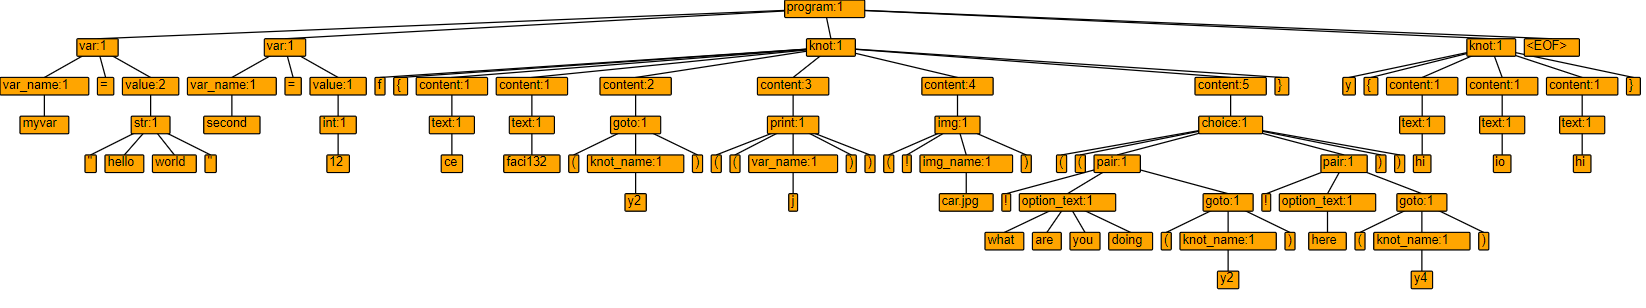
\includegraphics[width=\textwidth]{images/parsetree.png} }